\documentclass{exam}

\usepackage{listings}
\usepackage{amsmath}
\usepackage{forest}
\usepackage{subcaption}
\usepackage{hyperref}
\usepackage{tikz}
\usetikzlibrary{arrows.meta, positioning}


\printanswers

\begin{document}

\begin{center}
\fbox{\fbox{\parbox{5.5in}{\centering CSC 212 Practice Final Exam \\ Problems marked with (*) are challenging and problems marked with (**) are hard}}}
\end{center}

\vspace{5mm}
\makebox[0.95\textwidth]{Your Name:\enspace\hrulefill}

\begin{questions}

% --------------------------------------------------------------------------------

\question[10] Insert $1,10,3,13,8,0$ into an initially empty separate chaining hash table with capacity $7$ and hash function $h(k) = 3k \bmod 7$. Draw the table after the final insertion.  Assume insertions occur at the \textbf{front} of chains.

\begin{solutionorbox}[3.5in]
The final table is $[[0],[],[8,3,10],[3],[13],[],[],[]]$.
\end{solutionorbox}

\question[10] Insert $1,0,7,8,14,5,12$ into an initially empty linear probing hash table with capacity $7$ and hash function $h(k) = 3k \bmod 7$. Draw the table after the final insertion.

\begin{solutionorbox}[3in]
The final table is $[0,7,14,1,8,15,12]$.
\end{solutionorbox}

\clearpage

\question[10] (*) Design suitable hash functions $h_1(k)$ and $h_2(k)$ for a double hashing table with capacity $17$.

\begin{solutionorbox}[4in]
One possible answer is $h_1(k) = k \bmod 17$ and $h_2(k)= 1 + (k \bmod 16)$.
\end{solutionorbox}

\question[10] Consider a linear probing hash table with capacity $m$ and load factor $0.5$. In the worst case, how many probes are performed by \texttt{contains}?

\begin{solutionorbox}[3.5in]
In the worst case, all $\frac{m}{2}$ full slots are inspected, and $1$ empty slot, for a total of $\frac{m}{2} + 1$ slots.
\end{solutionorbox}

\clearpage

\question[10] Convert the following adjacency matrix to an adjacency list.
\begin{align*}
    \begin{bmatrix}
        0 & 1 & 1 & 1 & 1 \\
        0 & 0 & 1 & 0 & 0 \\
        0 & 0 & 1 & 0 & 0 \\
        0 & 0 & 1 & 0 & 0 \\
        1 & 1 & 1 & 1 & 0 
    \end{bmatrix}
\end{align*}

\begin{solutionorbox}[2.5in]
The adjacency list is $[[1,2,3,4], [2], [2], [2], [0,1,2,3]]$.
\end{solutionorbox}

\question[10] Give the adjacency matrix for the following graph.

\begin{center}
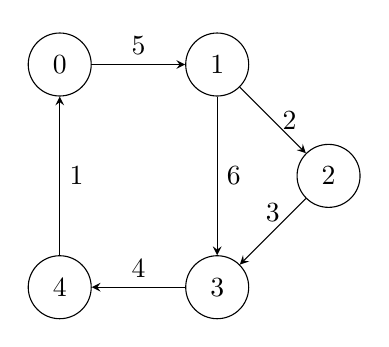
\begin{tikzpicture}[>=stealth, node distance=2cm]
    \tikzstyle{n}=[circle, draw, minimum size=8mm]

    \node[n] (0) {0};
    \node[n, right of=0] (1) {1};
    \node[n, below right of=1] (2) {2};
    \node[n, below left of=2] (3) {3};
    \node[n, left of=3] (4) {4};
    
    \draw[->] (0) -- node[midway, above] {5} (1);
    \draw[->] (1) -- node[midway, right] {2} (2);
    \draw[->] (2) -- node[midway, above] {3} (3);
    \draw[->] (3) -- node[midway, above] {4} (4);
    \draw[->] (4) -- node[midway, right] {1} (0);
    \draw[->] (1) -- node[midway, right] {6} (3);
\end{tikzpicture}
\end{center}

\begin{solutionorbox}[2.5in]
The adjacency matrix is
\begin{align*}
    \begin{bmatrix}
        0 & 5 & 0 & 0 & 0 \\
        0 & 0 & 2 & 6 & 0 \\
        0 & 0 & 0 & 3 & 0 \\
        0 & 0 & 0 & 0 & 4 \\
        1 & 0 & 0 & 0 & 0
    \end{bmatrix}
\end{align*}
\end{solutionorbox}

\clearpage

\question[10] Find the lexicographically smallest depth-first traversal of the following graph.

\begin{center}
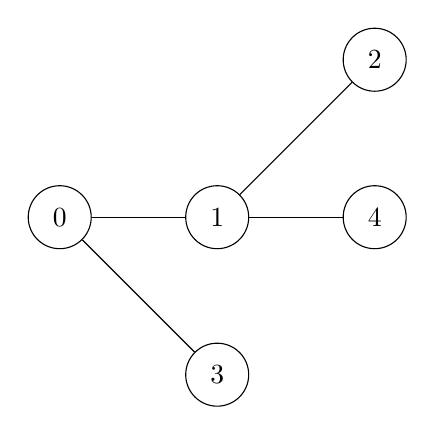
\begin{tikzpicture}[>=stealth, node distance=2cm]
    \tikzstyle{n}=[circle, draw, minimum size=8mm]

    \node[n] (0) {0};
    \node[n, right of=0] (1) {1};
    \node[n, right of=1] (4) {4};
    \node[n, above of=4] (2) {2};
    \node[n, below of=1] (3) {3};
    
    \draw (0) -- (1);
    \draw (1) -- (2);
    \draw (1) -- (4);
    \draw (0) -- (3);
\end{tikzpicture}
\end{center}

\begin{solutionorbox}[1in]
The lexicographically smallest depth-first traversal is $0,1,2,4,3$.
\end{solutionorbox}


\question[10] (**) Consider a social media platform where users can have \textbf{mutual friends}. That is, if user $A$ is friends with user $B$, user $B$ is also friends with user $A$. 

We say users $A$ and $B$ are \textbf{indirect friends} if $A$ is friends with $B$ or one of $A$'s friends is an indirect friend of $B$. A \textbf{community} is a set of users where every pair of users are indirect friends and no users have indirect friends outside of the community. 

Describe how to model friendships as a graph, clearly defining the vertices and edges. Give pseudocode for computing the total number of communities.

\begin{solutionorbox}[3.5in]
The vertices are users. There is an edge between two vertices if and only if the corresponding users are friends. To compute the total number of communities
\begin{enumerate}
    \item Create an empty set to track visited vertices, and an counter initialized to zero.
    \item For each vertex $v$,
    \begin{enumerate}
        \item If $v$ is already visited, skip it.
        \item Otherwise, run a DFS starting at $v$ that marks all traversed vertices as visited. Increment the counter by one.
    \end{enumerate}
    \item Return the counter.
\end{enumerate}
\end{solutionorbox}

\clearpage


\question[10] (*) An \textbf{RL-rotation} is equivalent to a right rotation on the root's right child, followed by a left rotation on the root.

Implement the \texttt{rl\_rotate} function. Assume that an RL-rotation on the subtree rooted by \texttt{root} is always valid. Return the new root after rotation. Your implementation must run in $\mathcal{O}(1)$ time.

\begin{center}
\begin{lstlisting}[language=C++]
struct Node {
    Node* left;
    Node* right;
    // ...
};

Node* rl_rotate(Node* root) {
    // TODO: Implement this function.
    
}
\end{lstlisting}
\end{center}

\begin{solutionorbox}[6in]
\begin{center}
\begin{lstlisting}[language=C++]
struct Node {
    Node* left;
    Node* right;
    // ...
};

Node* rl_rotate(Node* root) {
    auto z = root;
    auto x = z->right;
    auto y = x->left;
    auto b = y->left;
    auto c = y->right;
    y->left = z;
    y->right = x;
    z->right = b;
    x->left = c;
}
\end{lstlisting}
\end{center}
\end{solutionorbox}

% --------------------------------------------------------------------------------

\clearpage

\question[10] Insert $0,1,2,3,4,5,6,7$ into an initially empty red-black tree. Draw the resulting tree, including colors, after each insertion. 

\begin{solutionorbox}[8in]
Check with \url{https://www.cs.usfca.edu/~galles/visualization/RedBlack.html}.
\end{solutionorbox}

% --------------------------------------------------------------------------------


\end{questions}

\end{document}